\documentclass{standalone}

\usepackage{tikz}
\usepackage{tkz-euclide}
\usetikzlibrary{calc}
\usetikzlibrary{positioning}
\usetikzlibrary{arrows.meta}

\usepackage{times}


\begin{document}
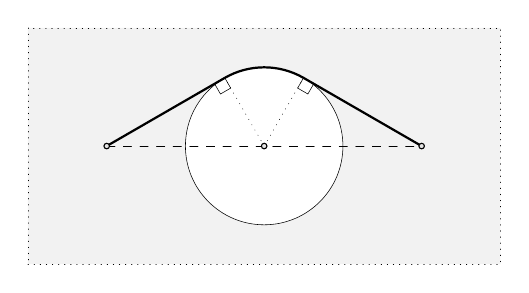
\begin{tikzpicture}[%
  >={Stealth[scale=1.0]},
  scale=1.0,
  % yscale=0.8,
]

  \tkzDefPoint(-3.0, -1.5){A}
  \tkzDefPoint(3.0, -1.5){B}
  \tkzDefPoint(3.0, 1.5){C}
  \tkzDefPoint(-3.0, 1.5){D}

  \tkzDrawPolygon[dotted,color=black,fill=black!5](A,B,C,D)

  \tkzDefPoint(0.0, 0.0){M}
  \tkzDefCircle[R](M,1.0)\tkzGetPoint{tmp}
  \tkzDrawCircle[draw=black,fill=white](M,tmp)

  \tkzDefPoint(-2.0, 0.0){p}
  \tkzDefPoint(2.0, 0.0){q}

  \tkzDefLine[tangent from = p](M,tmp)\tkzGetPoints{l1}{l2}
  \tkzDefLine[tangent from = q](M,tmp)\tkzGetPoints{r1}{r2}

  \tkzDrawSegments[thick](p,l1 r2,q)
  \tkzDrawArc[thick](M,r2)(l1)

  \tkzDrawSegment[dashed](p,q)
  \tkzDrawSegments[dotted](M,l1 M,r2)
  \tkzMarkRightAngle[very thin,size=0.15](M,l1,p)
  \tkzMarkRightAngle[very thin,size=0.15](M,r2,q)

  \tkzDrawPoints(p,q,M)

\end{tikzpicture}
\end{document}
